\section{What's the angle between your vertebrae?\\ \small{(%Pathway: Any; 
Pre-requisite: None)}}
%\item
%\underline{\large\bf Measuring angles on X-ray images}  \\[0.1cm]
\begin{minipage}{9.5cm}
Using X-rays, one can measure angles between bones in a body (e.g., between
two vertebrae, as shown on the X-ray of a model with pins [1]). However, when
measuring an angle on an image, the result may not be the same as the true
angle. Thus, in the diagram below the angle $\varphi $ that an object
(``stick'' of length $l$) makes with the horizontal, is not necessarily equal
to the angle $\psi $ between its image I and the horizontal line on the
screen.
\end{minipage}
\hspace{0.3cm}
\begin{minipage}{6.5cm}
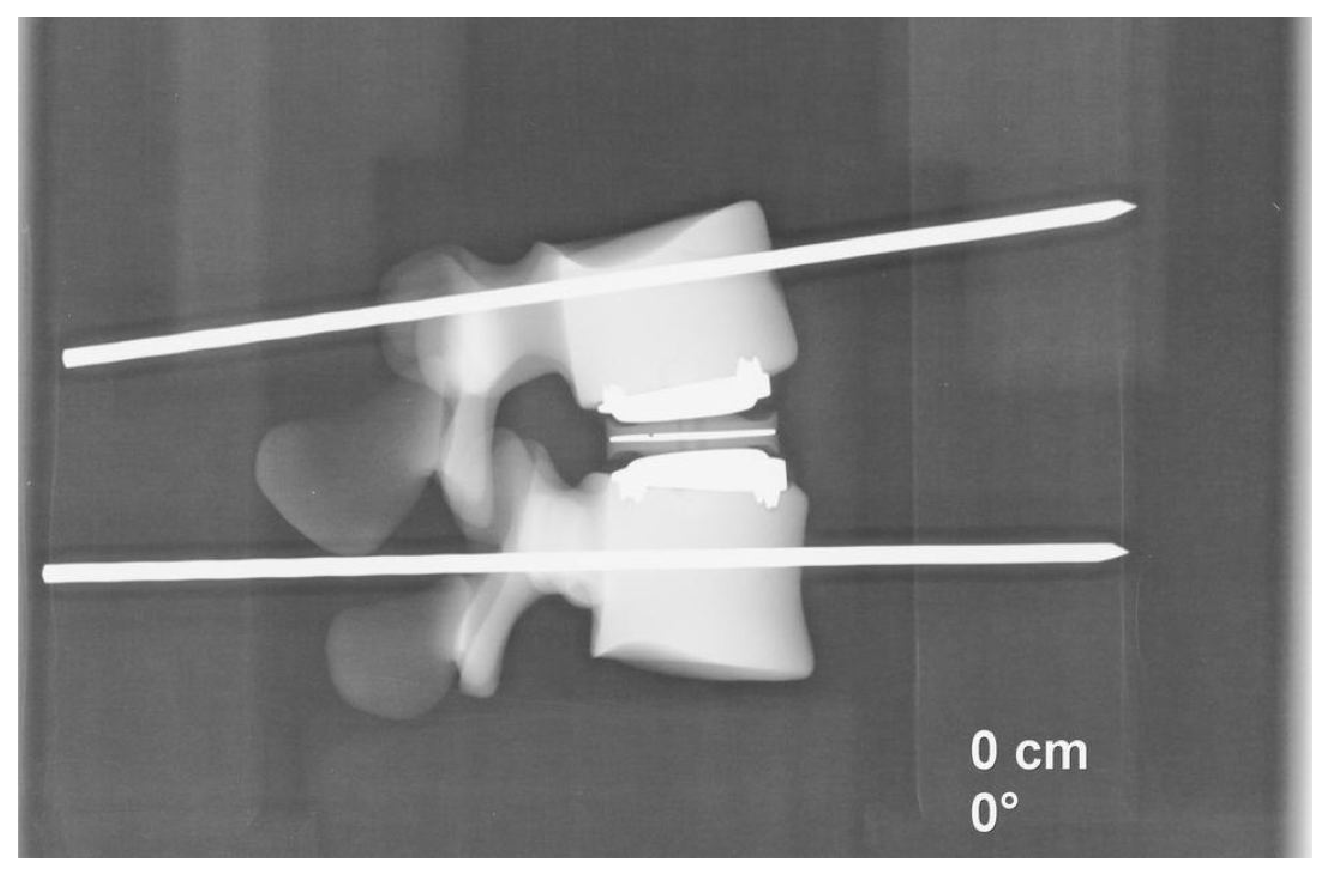
\includegraphics[angle=0,width=6.5cm]{projects/Vertebrae_image.eps}
\end{minipage}

\begin{center}
%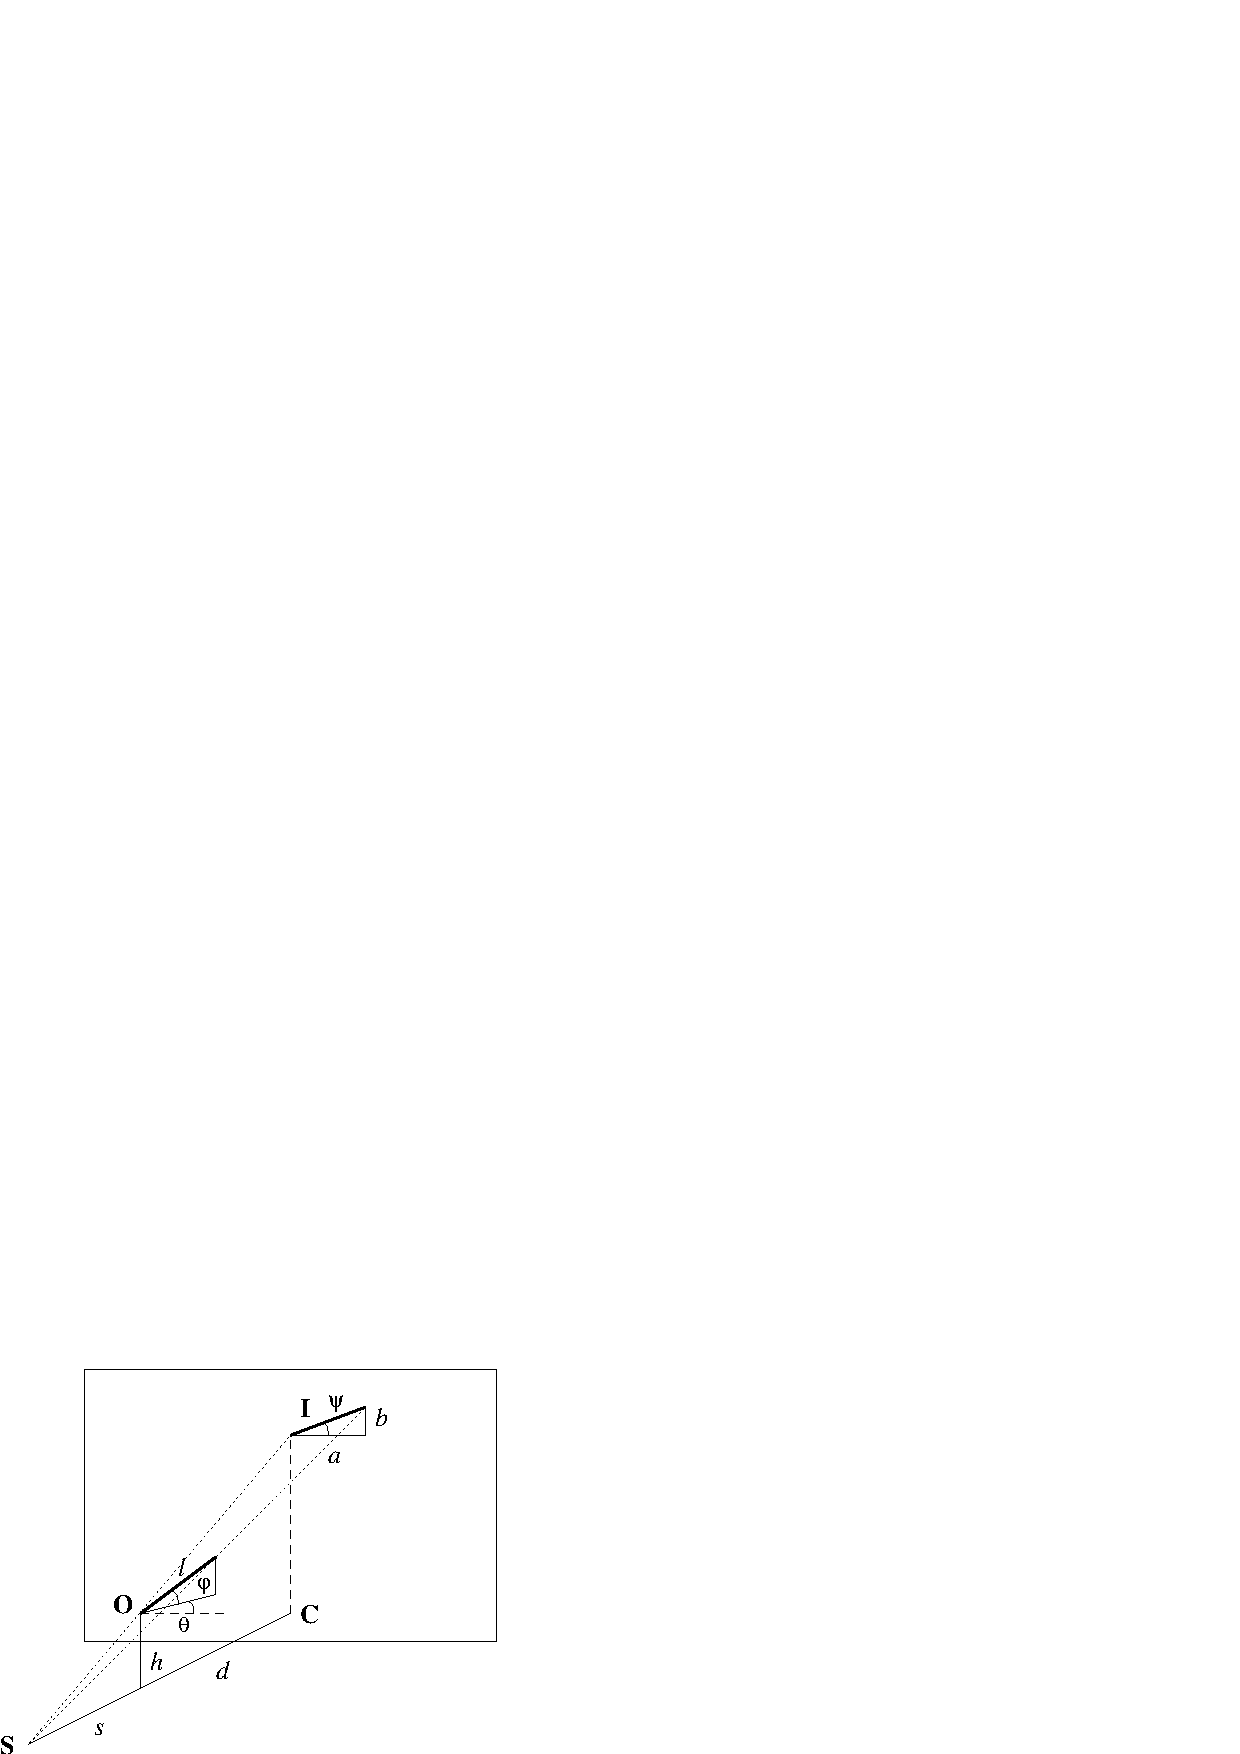
\includegraphics[width=10cm,angle=-90]{X_ray.pdf}
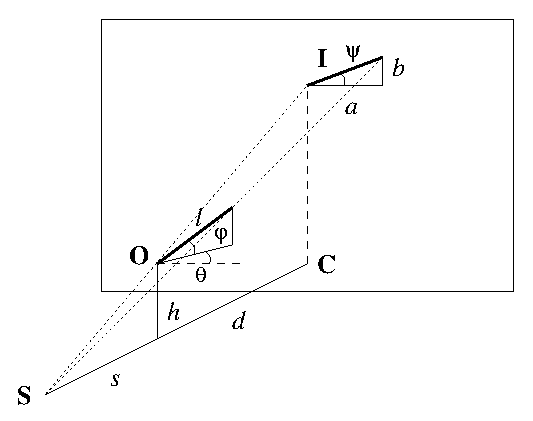
\includegraphics[width=8cm]{projects/X_ray.eps}
\end{center}

The difference between $\varphi $ and $\psi $ may depend on the
distance $s$ between the X-ray source S and the plane
parallel to the screen which contains one end of the object O,
and the distance $d$ between O and the plane of the screen.
It may also depend on the height $h$ of the end-point O
above the line SC perpendicular to the screen, and on the
angle $\theta $ that the vertical plane through O makes
with the direction parallel to the screen.\\[6pt]
Using the above diagram or otherwise, show that
\begin{equation}
\tan \psi =\frac{1}{\cos \theta }\tan \varphi -\frac{h}{s}\tan \theta .
\end{equation}
Investigate how the difference beteeen $\psi $ and $\varphi $ depends on the
angle $\theta $ and the vertical displacement $h$.\\[6pt]
You can further investigate if one can find $\varphi $ from the results of
two measurements (yielding $\psi _1$ and $\psi _2$), corresponding to two
position $\theta _1$ and $\theta _2$, for which only the difference
$\Delta \theta =\theta _2-\theta _1$ is known.\\[6pt]
[1] John McManus, {\em The Influence of X-Ray Technique on the Angle
Measurement of an Artificial Disc}, Thesis (Queen's University Belfast, 2006).
%thesis(unpublished).
%In this work X-rays were taken of model vertebrae which had metal pins
%inserted in them for the purpose of measuring the angles more accurately
%(something that would be hard to do on a real patient!).
